\chapter{BPA数据读取}

\section{BPA数据卡片的分类}

主要的数据卡片可分为四类,分别为区域控制、节点数据、支路数据及节点数据修改卡。

\begin{table}[h]
\centering
\begin{tabular}{ll}
\toprule
卡片分类 & 卡片描述\\
\midrule
 区域控制数据卡 & AC、A,指定参与区域功率交换的分区及安排交换功率量 \\ 
 & AO,按区域分类输出 \\ 
 & I,指定区域交换功率 \\ 
 \midrule
 节点数据卡 & B,交流节点卡\\
 & BD,两端直流节点卡\\
 & BM,多端直流节点卡\\
 & +,延续节点卡\\
 & X,可切换电抗、电容器卡\\
 \midrule
 支路数据卡 & L,对称线路卡\\
 & LD,两端直流线路卡\\
 & LM,多端直流线路卡\\
 & T,变压器和移相器卡\\
 & R,带负荷调压变压器调节数据卡\\
 & E,不对称等值支路卡\\
 & RZ,可快速调整的线路串补数据卡\\
 \midrule
 数据修改卡 & P,系统中发电出力和负荷按百分数修改卡\\
 & Z,分区重新命名卡\\
 & DZ,分区删除卡\\
\bottomrule
\end{tabular}
\caption{主要数据卡片分类}
\end{table}

在BPA到DIgSILENT的数据转换程序中,我们需要处理的主要是一下这些卡片:B,交流节点卡;L,对称线路卡;T,变压器和移相器卡;P,系统中发电出力和负荷按百分数修改卡。下面来详细介绍各个卡片的数据格式和模型。

\section{B卡}

\begin{figure}[H]
\centering
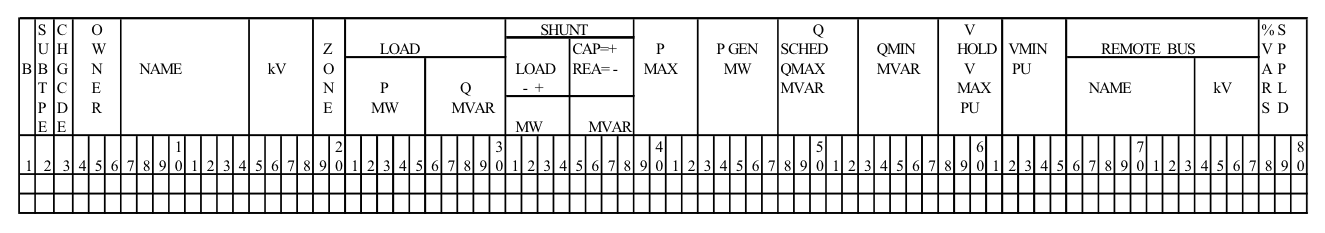
\includegraphics[width=1.05\textwidth]{images/Paper_Fig_17.png}
\setcaptionwidth{\linewidth}
\caption{B卡数据}
\end{figure}

\begin{spacing}{1.0}
\begin{longtable}[h]{llp{0.85\columnwidth}}
\toprule
列 & 格式 & 内容\\
 \midrule
1 & A1 & 卡片类型-B\\
 & A1 & 卡片子型-各子型如下: \\ 
 & & 空白-PQ节点\\ & &
T-PQ节点,但节点电压受带负荷调压变压器控制\\ & &
C-PQ节点,但节点电压受某发电机控制\\ & &
V-PQ节点,但节点电压有限制值:$V_{min}<V<V_{max}$,当电压越界
时,自动转换为PV节点,这时Q起变化,以保证电压在限制值
内,由此产生的未安排	无功,将由程序自动装上电容器(电抗
器)来平衡 \\ & &
E-PV节点,无功出力没有限制,但为达到控制电压,无功出力
超过上下限时,超过部分无功称为未安排无功,程序自动装上电
容器或电抗器 \\ & &
Q-PV节点,但节点无功功率有限制值:$Q_{min}<Q<Q_{max}$,当越界
时,自动转换为PQ节点 \\ & &
G-PV节点(其为发电机节点),缺省电压在0.95~1.15之间变
化,并去控制BC节点的电压。其无功Q也有限制,当Q越限时,中
止电压控制。被控节点不可以是Vθ节点、BG节点或者其它已处
于被控状态下的节点 \\ & &
F-在计算中先作为PV节点,待有功功率P收敛后再自动转换为B
(PQ)节点 \\ & &
S-Vθ节点,为交流同步网的缓冲机 \\ & &
J-在采用改进的牛顿-拉夫逊法时作为BS节点,当解法转化为牛
顿-拉夫逊法以后,该节点自动转换为B(PQ)节点 \\ & &
K-在采用改进的牛顿-拉夫逊法时作为BS节点,当解法转化为牛
顿-拉夫逊法以后,该节点自动转换为BE(PV)节点 \\ & &
L-在采用改进的牛顿-拉夫逊法时作为BS节点,当解法转为牛顿-
拉夫逊法以后,该节点自动转换为BQ(PV节点,$Q_{min}\leqslant Q\leqslant
Q_{max}$)节点 \\ & &
X-在该节点装有电抗器或者电容器,由程序自动控制投切电抗器
或者电容器,以维持该节点或者其它节点的电压为给定值。\\
 
\bottomrule
\end{longtable}
\end{spacing}

其中S节点的判断比较重要,需要特殊处理。需在同步电机卡中选定为reference machine,如图5.1所示。

\begin{figure}[H]
\centering
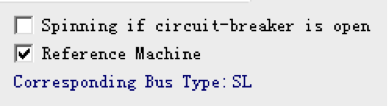
\includegraphics[width=0.6\textwidth]{images/Paper_Fig_18.png}
\setcaptionwidth{\linewidth}
\caption{reference machine选择}
\end{figure}

\subsection{DIgSILENT负载模型介绍及数据转换}

\begin{spacing}{1.0}
\begin{longtable}[h]{llp{0.8\columnwidth}}
\toprule
列 & 格式 & 内容\\
 \midrule
2 & A1 & 修改码,在程序中不做处理\\
4-6 & A3 & 所有者代码-用于确定区域功率交换中联络线的测点和输出表中按所有者分类的分析报告,可不填,当不填时在DIgSILENT中选取为0号owner。 \\ 
7-18 & A8, F4.0 & 节点名称(7-14),此节点名称直接设这为DIgSILENT节点ElmTerm项的NAME,而基准电压(kV)(15-18)则直接设定为DIgSILENT的Nominal Voltage(标准电压)。\\
19-20 & A2 & 节点所在的分区名称,在区域功率交换中用于确定区域的分区,在系统合并和按分区分类输出时也有用。在转换到DIgSILENT的过程中作为网络数据的大框架,使所有节点,线路,变压器等元器件都转换在这项之下。\\
\textbf{21-30} & \textbf{2F5.0} & \textbf{以MW和Mvar表示的恒定负荷,无功正值为感性、负值为容性。这两项数据正是该节点负载的数据信息。}\\
\bottomrule
\end{longtable}
\end{spacing}

如上表所示,第21-30列为描述恒定负荷所需要的有功、无功信息,在DIgSILENT中对应的是负载模型。

\begin{figure}[H]
\centering
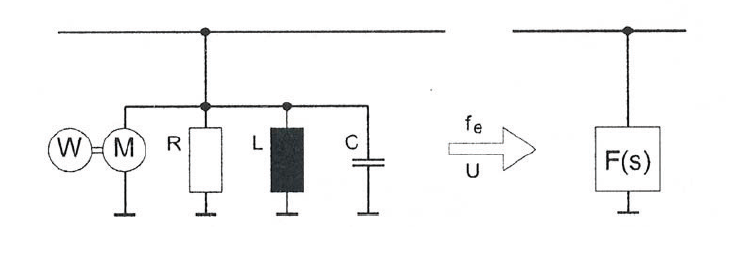
\includegraphics[width=1.0\textwidth]{images/Paper_Fig_19.png}
\setcaptionwidth{\linewidth}
\caption{DIgSILENT普通负载模型}
\end{figure}

DIgSILENT中采用的负荷模型是一种动态负荷、静态负荷与用户自定义“特殊”负荷的综合,在DIgSILENT中负载模型描述如图5.3.

通常情况下选择为3项平衡负载,切数据输入模式(Input Mode)选择为Default模式。在平衡负载情况之下,负载的潮流分析可不用专门将其专门设为单相或双相负载。其潮流模型如下:

\begin{figure}[H]
\centering
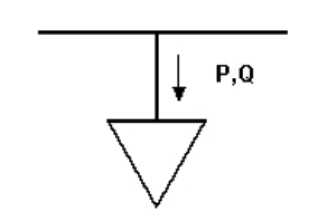
\includegraphics[width=0.4\textwidth]{images/Paper_Fig_20.png}
\setcaptionwidth{\linewidth}
\caption{DIgSILENT平衡负载的潮流模型}
\end{figure}

负荷电压依赖性可以如下述方程建模:
$$P = P_0\left[aP*(\frac{v}{v_0})^{e\_ap} + bP*(\frac{v}{v_0})^{e\_bp} + cP*(\frac{v}{v_0})^{e\_cp}\right] \eqno{(5.1)}$$
其中
$$1 - aP - bP = cP \eqno{(5.2)}$$
$$Q = Q_0\left[aP*(\frac{v}Q{v_0})^{e\_aQ} + bQ*(\frac{v}{v_0})^{e\_bQ} + cQ*(\frac{v}{v_0})^{e\_cQ}\right] \eqno{(5.3)}$$
其中
$$1 - aQ - bQ = cQ \eqno{(5.4)}$$

\begin{center}
\begin{table}[h]
\centering
\begin{tabular}{p{0.2\columnwidth}p{0.2\columnwidth}}
\toprule
指数 & 常量\\
\midrule
 0 & 功率\\
 1 & 电流\\
 2 & 电阻\\
\bottomrule
\end{tabular}
\caption{为实现不同负载功效的指数选取}
\end{table}
\end{center}


通过对上述公式的几项指数经行赋值,就可以对固有的负载建模。表5.4提供了分别实现恒功率,恒电流以及恒定电阻特性的负载模型所需要的指数参数。但是相应的每个系数($aP, bP, cP, aQ, bQ, cQ$)则可以任意定义如图:

\begin{figure}[H]
\centering
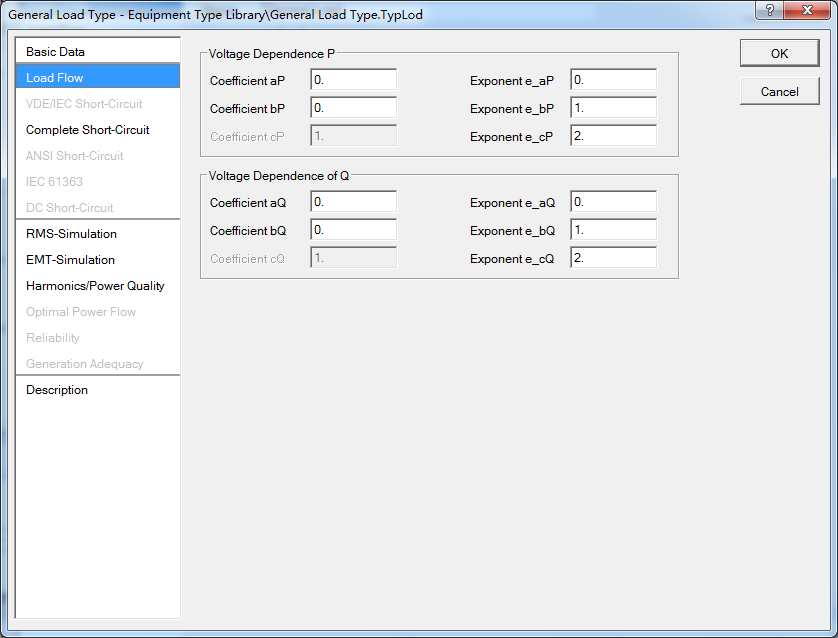
\includegraphics[width=0.9\textwidth]{images/Paper_Fig_21.png}
\setcaptionwidth{\linewidth}
\caption{不同功能负载实现的系数表格图}
\end{figure}

如图5.5所示,以有功功率为例,图中的参数使得有功负载的最后方程形式为$P = P_0\left[aP*(\frac{v}{v_0})^0 + bP*(\frac{v}{v_0})^1 + cP*(\frac{v}{v_0})^2\right]$,可见负载有功不仅与恒定功率$P_0$有关,还与负载电压平方有关,而且负载功率受电压控制,这正好与$P = \frac{U^2}{R}$公式一致,所以当取$aP = bP = aQ = bQ = 0$,$cP = cQ = 1$时可以表示为一恒阻抗负荷,即可以作为一个阻抗使用。

同理,当取$aP = aQ = 1$,$bP = bQ = 0$,$cP = cQ = 0$时,则是恒功率负载。

通过负荷调节因子,负载可以单独被放大或者缩小如下:

$$P = scale * P_0 \eqno{(5.5)}$$
$$Q = scale * Q_0 \eqno{(5.6)}$$
$$P = scale * P_0\left[aP*(\frac{v}{v_0})^{e\_ap} + bP*(\frac{v}{v_0})^{e\_bp} + cP*(\frac{v}{v_0})^{e\_cp}\right] \eqno{(5.7)}$$
$$Q = scale * Q_0\left[aP*(\frac{v}Q{v_0})^{e\_aQ} + bQ*(\frac{v}{v_0})^{e\_bQ} + cQ*(\frac{v}{v_0})^{e\_cQ}\right] \eqno{(5.8)}$$

公式5.7和5.8是考虑到有电压依赖的情况下的特性。

当考虑到馈线负荷调节过程中的负载,则在DIgSILENT的\emph{ElmLod}数据卡中需要选定\emph{“Adjusted by Load Scaling”},这种情况下潮流计算时数据卡中本身的范围因素将不被使用而是被feeder-scaling因素给替换,如图5.6显示了负荷调节因子用以维持feeder设置的方式。

\begin{figure}[H]
\centering
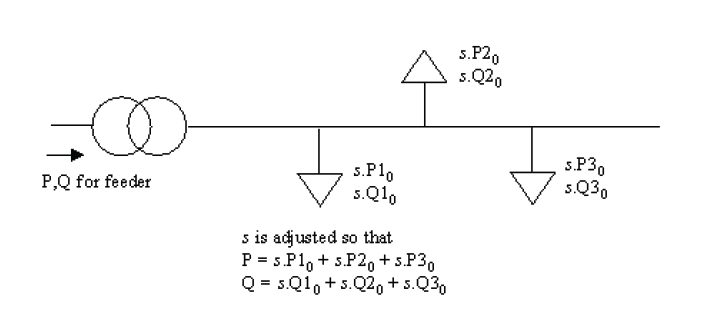
\includegraphics[width=0.9\textwidth]{images/Paper_Fig_22.png}
\setcaptionwidth{\linewidth}
\caption{负荷调节因子用以维持feeder设置的方式}
\end{figure}

以上是DIgSILENT负载潮流特性的参数介绍,对于数据的转换由于BPA只给出了负载的有功和无功所以最主要的是将有功和无功分别准确的转化DIgSILENT有功无功的输入项$P_0, Q_0$。对应的DIgsILENT数据位置如图5.7所示。

\begin{figure}[H]
\centering
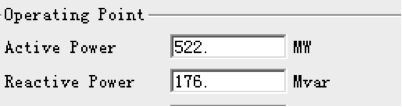
\includegraphics[width=0.6\textwidth]{images/Paper_Fig_23.png}
\setcaptionwidth{\linewidth}
\caption{负载有功,无功的转换}
\end{figure}

\subsection{DIgSILENT电抗器模型介绍及数据转换}

\begin{spacing}{1.0}
\begin{longtable}[h]{llp{0.8\columnwidth}}
\toprule
列 & 格式 & 内容\\
 \midrule
31-38 & 2F4.0 & 以MW和Mvar表示的、在基准电压下的节点并联导纳负
荷,无功:(+)=容性,(-)=感性。注意:对于BX节点,此项忽略\\
\bottomrule
\end{longtable}
\end{spacing}

R-L型电抗器:此种电抗器是电阻与电感串联构成的。为了定义电感以及电阻需要两种输入模式:

\begin{description}
\item[-] 设计参数:参数通过额定无功功率,额定电流和品质因数确定。
\item[-] 布线参数:参数通过感抗和电阻确定。
\end{description}

式5.9给出了电感L与感抗的一般关系:
$$L_{rea} = \frac{X_{rea}}{2 \pi f_{nom}} \cdot 1000 \eqno{(5.9)}$$

\begin{figure}[H]
\centering
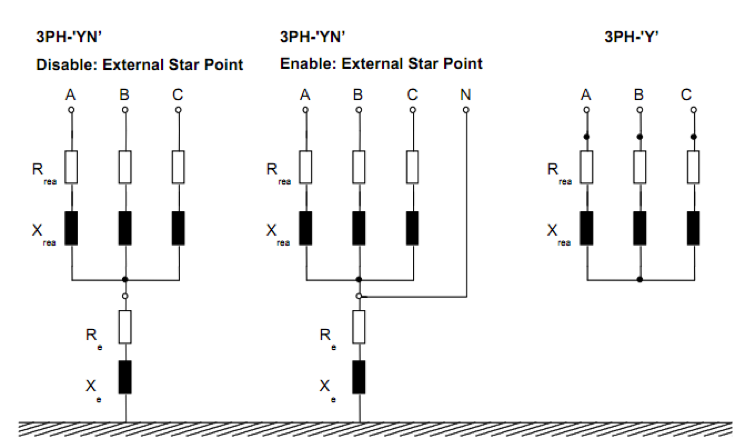
\includegraphics[width=0.9\textwidth]{images/Paper_Fig_24.png}
\setcaptionwidth{\linewidth}
\caption{\emph{3PH-'YN',3PH-'Y'}技术模型}
\end{figure}

如图5.8所示为\emph{3PH-'YN',3PH-'Y'}技术,如果内部接地阻抗星型点已经\emph{'connected'},可以将星型接法的接线点连接到中性线路(建立方式:\emph{External Star Point)}来建立\emph{'connected'}(如图2-12的二图情况)。对于中心点连接的情况,接地电阻和接地感抗需要考虑(如图2-12的一图情况),对于\emph{'disconnected'}情况,接地电阻和感抗可以忽略。

$X_{rea}, R_{rea}, Q_{rea}$的关系如式5.10和5.11所示,其中$qf_{rea}$是额定频率下的品质因数。
$$X_{rea} = \frac{U_{nom}^2}{Q_{rea}} \eqno{(5.10)}$$
$$R_{rea} = \frac{X_{nom}}{qf_{rea}} \eqno{(5.11)}$$

电抗器无功功率与额定电流关系如下:
$$Q_{rea} = \frac{I_{rea}\cdot \sqrt{3}\cdot U_{nom}}{1000} \eqno{(5.12)}$$
$$\Delta S = \Delta P + j\Delta Q = 3I^2(R + jX) = \frac{P^2 + Q^2}{U^2_j}(R + jX) \eqno{(5.13)}$$

另一种电抗器是C型电抗器:此种电抗器是纯电容型的。有两种模式可以定义C型电容器:

\begin{description}
\item[-] 设计参数:参数通过额定电容功率,额定电流。
\item[-] 布线参数:参数通过容抗和电容确定。
\end{description}

电容和电抗的关系如式5.14所示:
$$C_{rea} = \frac{B_{rea}}{2 \cdot \pi \cdot f_{rea}} \eqno{(5.14)}$$

如图5.9所示,在\emph{ABC-'YN',ABC-'Y'}技术中,如果内部接地阻抗星型点已经\emph{'connected'},可以将星型接法的接线点连接到中性线路(建立方式:\emph{External Star Point})来建立\emph{'connected'}(如图2-13的二图情况)。对于中心点连接的情况,接地电阻和接地感抗需要考虑(如图2-13的一图情况),对于\emph{'disconnected'}情况,接地电阻和感抗可以忽略。

\begin{figure}[H]
\centering
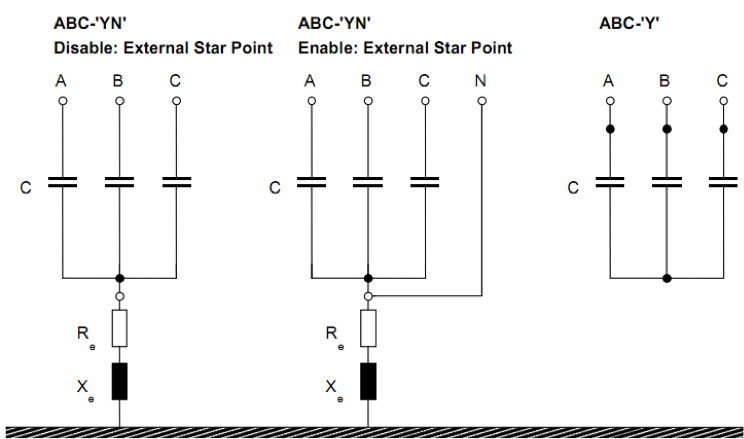
\includegraphics[width=0.9\textwidth]{images/Paper_Fig_25.png}
\setcaptionwidth{\linewidth}
\caption{\emph{ABC-'YN',ABC-'Y'}技术模型}
\end{figure}

$B_{cap}$和$Q_{cap}$的关系以及$Q_{cap}$和$I_{cap}$的关系分别如式5.15和5.16所示:
$$B_{cap} = \frac{Q_{cap}}{U_{nom}^2} \cdot 10^6 \eqno{(5.15)}$$
$$Q_{cap} = \frac{I_{cap} \cdot \sqrt{3} \cdot U_{nom}}{1000} \eqno{(5.16)}$$

R-L-C型电抗器:它由感抗,电阻,容抗串联构成。为了定义其感抗,电阻以及容抗,有两种输入模式:

\begin{description}
\item[-] a)设计参数:参数通过额定有功功率(L-C),额定电流(L-C),电感等级或共振频率或者调谐顺序以及额定频率下的品质因数或者共振频率下的品质因数。
\item[-] 布线参数:参数通过感抗或者电感,容抗或者电容大小以及电阻确定。
\end{description}

容抗$B_{cap}$和电容$C_{cap}$的关系如式5.17所示。
$$C_{cap} = \frac{B_{cap}}{2 \cdot \pi \cdot f_{nom}} \eqno{(5.17)}$$

感抗$X_{rea}$和电感$L_{rea}$的关系如式5.18所示。
$$L_{rea} = \frac{X_{rea}}{2\cdot \pi \cdot f_{nom}} \cdot 1000 \eqno{(5.18)}$$

电感等级,共振频率以及调谐顺序关系如下式所示,其中$P_{grad}$是电感度。
$$f_{res} = \frac{f_{nom}}{\sqrt{P_{grad} / 100}} \eqno{(5.19)}$$
$$n_{res} = \frac{f_{res}}{f_{nom}} \eqno{(5.20)}$$

如式5.21所示为额定频率下的品质因数与共振频率下品质因数的关系。
$$g_{reaf_{0}} = g_{rea} \cdot n_{res} = g_{rea} \cdot \frac{f_{res}}{f_{nom}} \eqno{(5.21)}$$

$g_{rea}$为额定频率下的品质因数,$g_{reaf_{0}}$为共振频率下的品质因数。

电容额定功率和额定无功功率,$L-C Q_{tot}$之间的关系如下:
$$Q_{cap} = Q_{tot} \cdot (1 - P_{grad} / 100) = Q_{tot} \cdot \left(1 - \left(\frac{f_{nom}}{f_{res}}\right)^2\right) \eqno{(5.22)}$$

$Q_{cap}$为额定电容功率,$Q_{tot}$为额定无功功率。

额定电感功率与额定无功功率,$L-C Q_{tot}$之间的关系如下:
$$Q_{cap} = Q_{tot} \cdot (100 / P_{grad} - 1) = Q_{tot} \cdot (n^2 - 1) = Q_{tot} \cdot \left(\left(\frac{f_{nom}}{f_{res}}\right)^2 - 1 \right) \eqno{(5.23)}$$

共振频率$f_{res}$由下式给出:
$$f_{res} = \frac{1}{2\pi \sqrt{L_{rea} \cdot 10^{-3} \cdot C_{cap} \cdot 10^{-6}}} \eqno{(5.24)}$$

电感,共振频率及电感之间的关系如下:
$$L_{rea} = \frac{10^3}{(2\pi f_{res}) \cdot C_{cap} \cdot 10^{-6}} \eqno{(5.25)}$$

$Q_{cap}$和$B_{cap}$之间的关系以及$X_{rea}, R_{rea}, Q_{rea}$三者之间的关系如下:
$$B_{cap} = \frac{Q_{cap}}{U_{nom}^2}\cdot 10^6 \eqno{(5.26)}$$
$$X_{rea} = \frac{U_{nom}^2}{Q_{rea}} \eqno{(5.27)}$$
$$R_{rea} = \frac{X_{rea}}{qf_{rea}} \eqno{(5.28)}$$

其中$qf_{rea}$是电阻设定为零的零的品质因数的品质因数。

以上就是对于DigSILENT中电抗器的介绍,但是上述的关键信息$qf_{rea}$在B卡中并没有给出,因此需要通过下述方法求出$qf_{rea}$。
$$I_{rea} = \frac{Q_[rea]}{\sqrt{2} \cdot U_{nom}} \cdot 1000 \eqno{(5.29)}$$
$$R_{rea} = \frac{P_{rea}}{I_{rea}^2} \cdot 1000 \eqno{(5.30)}$$
$$qf_{rea} = \frac{X_{rea}}{R_{rea}} \eqno{(5.31)}$$

而且由于B卡只提供了电抗器的无功及有功功率,无法判别其到底是R-L还是R-L-C模型,所以一般情况下只区分B卡的电抗器是C还是R-L型。(另外值得注意的是,软件中的电压都是线电压)

\subsection{DIgSILENT同步发电机模型介绍及数据转换}

\begin{spacing}{1.0}
\begin{longtable}[h]{llp{0.8\columnwidth}}
\toprule
列 & 格式 & 内容\\
 \midrule
39-42 & F4.0 & $P_{max}$:最大有功出力(MW)\\
43-47 & F5.0 & $P_{gen}$:实际有功出力(MW)\\
48-52 & F5.0 & 对于PQ节点(即B、BC、BT、BV节点)此项填所安排 的无功出力值QSCHED(Mvar);对于其它节点此项填无功出力 最大值$Q_{max}$(Mvar):(+)=容性,(-)=感性\\
53-57 & F5.0 & 无功出力最小值$Q_{min}$(Mvar)\\
58-61 & F4.3 & 所安排的电压值或者$V_{max}$(标么值)\\
62-65 & F4.3 & 所安排的$V_{min}$值(标么值),对于Vθ(即BS型)节 点,此项填角度值,注意此时省缺的格式为F4.1,单位度\\
66-77 & A8,F4.0  & 对于BG和BX节点有用,填写其所要控制的节点名(66- 73)和基准电压(74-77)。要控制的电压值填在被控节点记录卡 58-61列\\
78-80 & F3.0 & 发电机在对远方节点作电压控制时,提供的无功功率的百分数\\
\bottomrule
\end{longtable}
\end{spacing}

对于上面的39-65列,他们都实际上是DIgSILENT中ElmSym同步电机的数据,以下是对DIgSILENT同步电机模型的介绍。

通常情况下有两种典型的同步发电机:
\begin{description}
\item[-] 轮转子发电机以及涡轮转子发电机
\item[-] 突轴转子发电机
\end{description}

轮转子发电机模型使用在转轴以接近1500~3000转每分钟旋转。这种类型发电机通常运用于热电厂以及核电厂。转速在60到750转每分钟的低转速的同步发电机通常使用突轴转子发电机的模式,这种发电机通常使用在柴油和水能发电站。

下面两图是这两种模式发电机的截面图。这两图同时也展现了d轴和q轴的方向。
